\section{Measuring Tor's Current State of Resilience to BGP Attacks}
\label{hijack_interception_measurement}

In order to defend Tor against active BGP attacks launched by network-level adversaries, we start by investigating the vulnerability of the Tor network to BGP prefix attacks and quantifying how much of the Tor network would be affected. First, we look at how to evaluate the Tor network in terms of susceptibility to hijack attacks. Second, we extend the metric to quantify how resilient the Tor network is to prefix interception attacks by Tier 1 ASes. These steps help quantify how vulnerable the Tor network is to network-level adversaries in a novel way.  Specifically, we measure:
%The metric used helps enlighten the community about the state of the Tor network, in terms of how resilient the relays are to hijack attacks.  

\begin{itemize}
\item How resilient ASes that contain Tor relays are to prefix hijack attacks
\item How resilient ASes that contain Tor relays are to prefix interception attacks
\item How resilient ASes that contain Tor relays were in the Indosat prefix hijack in 2014
%\item Resiliency (to prefix hijack attacks) of the ASes that contain relays and compare the resiliency of ASes that contain more relays to those that contain few relays.
%\item Resiliency (to prefix interception attacks) of the ASes that contain relays and compare the resiliency of ASes that contain more relays to those that contain few relays.
%\item How much resiliency to hijacks and interceptions on the Tor network differs year to year, starting in 2008.
\end{itemize}

\subsection{Resilience to prefix hijack attacks}
\label{hijack_methodology}

Network-level adversaries can launch a BGP prefix hijack by announcing a prefix that it does not own. Consequently, some ASes would be deceived by the false announcement and thus send traffic to the false origin AS instead of the true origin AS. Previous work has tackled questions of AS resilience to prefix hijack attacks using simulations of the entire Internet \cite{lad2007understanding}.  We build off this work by applying these metrics to the Tor network. \cite{lad2007understanding} explains the probability of a node $v$ believing the true origin $t$ given a false origin $a$ announcing a route that belongs to true origin $t$:

\begin{equation}
\bar{\beta}(t,a,v) = \frac {p(v,t)} {p(v,t) + p(v,a)}
\end{equation}

where $p(v,a)$ is the number of equally preferred paths from node $v$ to false origin $a$ and $p(v,t)$ is the number of equally preferred paths from node $v$ to true origin $t$.  Using this probability, the resilience metric is introduced -- the resilience of a node $t$ is the fraction of nodes that believe the true origin $t$ given an arbitrary hijack against $t$:

\begin{equation}
R(t) = \sum_{a \in N} \sum_{v \in N} \frac {\bar{\beta}(t,a,v)} {(N-1)(N-2)}
\end{equation}

where N is the total number of ASes.

To measure the resilience of Tor-related ASes, we first use an Internet topology~\cite{caida} to get all of the AS relationships, and construct an AS-level graph.  We identify the Tor-related ASes and simulate prefix hijacks on the graph. Algorithm~\ref{algo:calcres} shows the steps we take on the AS graph to calculate the resilience of Tor-related ASes from a source AS $t$. Then, by summing the resilience values from \emph{all} source ASes and dividing by $(N-1)$, we get the total resilience of each Tor-related AS.
%Specifically, our methodology consists of:

%\begin{enumerate}
%\item Construct an AS-level graph from an Internet topology.
%\item Identify ASes that have at least one Tor guard/exit relay.
%\item Calculate the number of equally preferred paths from AS A to AS B, where AS B is a Tor-related AS.
%\item Calculate the number of equally preferred paths from AS A to AS C, where AS C is the attacking (hijacking) AS.
%\item Calculate resiliency using Equation (2).
%\end{enumerate}

%We follow this methodology for every AS A $\neq$ a Tor-related AS, every AS C $\neq$ a Tor-related AS, and for every AS B $=$ Tor-related AS.  

\begin{algorithm}
\caption{Algorithm to calculate prefix hijack resilience for Tor-related ASes.}
\label{algo:calcres}
\begin{algorithmic}
\Function{CalcResilience}{graph $G$, node $t$}
    \State \Call{CalcPathsFromNode}{$G,t$}
    \State $zeros(R)$
    \For{each reachable node $v$ from node $t$} 
    	\If{node $v$ contains Tor guard/exit relays}
		\State $n \gets $ num. of less preferred nodes than node $v$
		\State $R[v] \gets n + \bar{\beta}(v,a,t)$ $\forall$ equally preferred node a
	\EndIf
    \EndFor
    \State $N \gets$ num. of nodes in $G$
    \State \Return $[R[i] / (N-2)$ for each node $i$ in $R]$
\EndFunction
\end{algorithmic}
\end{algorithm}

Note that the $\Call{CalcPathsFromNode}{G,t}$ step computes paths from source AS $t$ to all other ASes, which requires AS-level path predictions. Previous works have shown that AS level paths are determined mainly based on two preferences ~\cite{gao2001stable}:

\begin{itemize}
\item Local Preference: customer route is preferred over peer route, which is preferred over provider route. 
\item Shortest Path: With the highest local preference, paths with the shortest hops will be preferred. 
\end{itemize}

Furthermore, the AS paths should also have the \emph{valley free} property ~\cite{gao2001inferring}. Thus, we use breadth first search to traverse the graph from a given source node based on this property and the preferences. We first explore provider-customer paths, which are the most preferred; next, we explore one peer-to-peer path followed by a sequence of provider-customer paths, which are the next preferred; finally, we explore customer-provider paths followed by an optional peer-to-peer path and then followed by a sequence of provider-customer paths. Note that, nodes are explored in the most preferred to least preferred order, and those which are explored in the same step are equally preferred. This ordering will help accelerate the resilience calculation. We will expand more details of our AS-level path prediction algorithm in Section~\ref{sec:discussion}. \yixin{add this to discussion}

%There is also space for metrics regarding specific relays' resiliency to BGP prefix hijack attacks, as well as metrics regarding BGP prefix interception attacks (AS- and relay-level).  

%  We also plan to specifically look at the resiliency of guard relays (as a group) as well as exit relays (as a group). 

\subsection{Resilience to prefix interception attacks}
\label{interception_methodology}
Next, we measure the resilience of Tor-related ASes to prefix interception attacks. Launching a prefix interception attack requires one further step than prefix hijack attacks - the false origin AS needs to forward the hijacked traffic back to the true origin AS. Prior work \cite{ballani2007study, pilosov16stealing} has pointed out that to be able to do this, the false origin AS needs to satisfy a \emph{safety condition}: none of the ASes along the existing route from false origin AS to true origin AS should choose the invalid route advertised by the false origin AS, and thus the false origin AS can still use its existing route to forward the hijacked traffic back to the true origin. Thus, when making the invalid route announcement, there are two cases to consider: (1) if the false origin AS's existing route to the true origin AS is through a peer or customer route, then it's safe to make the false announcement to all its neighbors without affecting its existing route to the true origin; (2) if the false origin AS's existing route to the true origin AS is through a provider route, then it can only make the false announcement to its peers and customers, but not providers. 

Based on the above property, we modify the Algorithm ~\ref{algo:calcres} to the following Algorithm~\ref{algo:calcintercept} to evaluate resilience to interception attacks. 

\begin{algorithm}
\caption{Algorithm to calculate prefix interception resilience for Tor-related ASes.}
\label{algo:calcintercept}
\begin{algorithmic}
\Function{CalcResilience}{graph $G$, node $t$}
    \State \Call{CalcPathsFromNode}{$G,t$}
    \State $zeros(R)$
    \For{each reachable node $v$ from node $t$} 
    	\If{node $v$ contains Tor guard/exit relays}
		\State $n \gets$ less preferred nodes than node $v$
		\If{existing route $t$ to $v$ is provider route}
			\State $n \gets (n - m)$ for all nodes $m$ for which $t$ to $m$ is provider route
		\EndIf
		\State $a \gets$ equally preferred nodes as node $v$
		\If{existing route $t$ to $v$ is provider route}
			\State $a \gets (a - m)$ for all nodes $m$ for which $t$ to $m$ is provider route
		\EndIf
		\State $R[v] \gets n + \bar{\beta}(v,a,t)$ $\forall$ equally preferred node a
	\EndIf
    \EndFor
    \State $N \gets$ num. of nodes in $G$
    \State \Return $[R[i] / (N-2)$ for each node $i$ in $R]$
\EndFunction
\end{algorithmic}
\end{algorithm}

%\begin{enumerate}
%\item Construct an AS-level graph from an Internet topology.
%\item Identify ASes that have at least one Tor relay.
%\item Calculate the number of equally preferred paths from AS A to AS B, where AS A $\neq$ AS B, AS A and AS B are not Tor-related ASes, and there must be a Tor relay on the path from AS A to AS B.
%\item Calculate the number of equally preferred paths from AS A to AS B, where AS A $\neq$ AS B, AS A and AS B are not Tor-related ASes, there must an AS C (intercepting AS) on the path from AS A to AS B, and no Tor-related AS on the path from AS A to AS B.
%\item Calculate resiliency using the equation described above.
%\end{enumerate}

\subsection{Hijack Resilience Results}

{\bf Resilience of the current Tor network.} We obtained the list of Tor relays from the Tor consensus data in January 2016 and retrieved their belonging ASes. Then, we downloaded the AS topology published by CAIDA in January 2016. The AS topology contains 52,838 ASes, in which 1,202 ASes contain a total of 6,942 Tor relays. We simulated \emph{all} possible hijacking scenarios against each of the 1,202 Tor-related ASes, totaling $52,837 \times 1,202 = 63,510,074$ prefix hijacks. We used the methods described in Section \ref{hijack_methodology} to evaluate the resilience of each Tor-related AS. 

\begin{figure}[ht!]
\centering
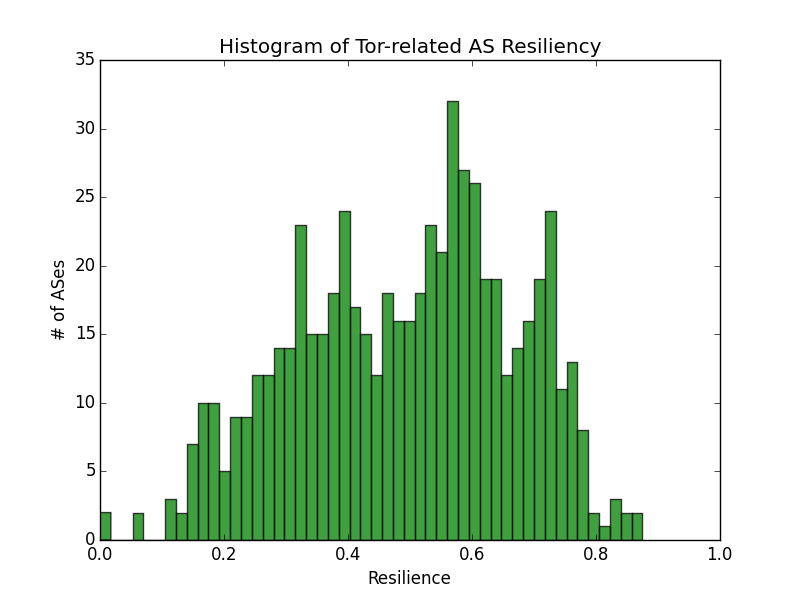
\includegraphics[width=.4\textwidth]{resilience_histogram}
\caption{Histogram of hijack resilience values for all Tor-related ASes.}
\label{fig:hijack_resilience_histogram}
\end{figure}

Figure~\ref{fig:hijack_resilience_histogram} shows the prefix hijack resilience results. We can see that most Tor-related ASes lie in the middle of the spectrum for resilience. We then look at AS resilience corresponding to its involvement in Tor in terms of number of Tor relays and aggregated Tor bandwidth that it contains. Figure ~\ref{fig:res_relays} shows the resilience value for an AS corresponding to the number of Tor relays it contains. Figure ~\ref{fig:hijack_bw} shows the resilience value for an AS corresponding to its total Tor bandwidth. 

\begin{figure}[ht!]
\centering
\begin{subfigure}{.25\textwidth}
  \centering
  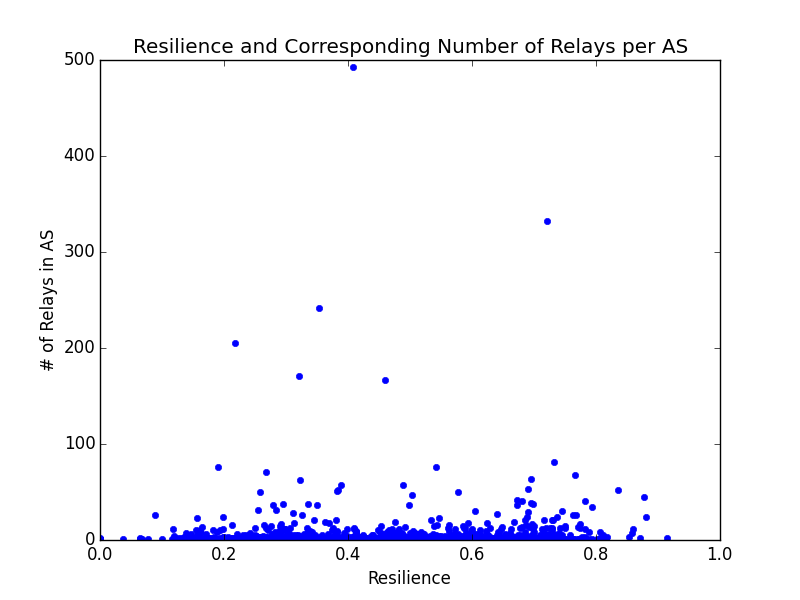
\includegraphics[width=\linewidth]{new_resilience_per_as}
  \caption{Hijack Resilience vs. Number of Tor Relays per AS}
  \label{fig:res_relays}
\end{subfigure}%
\begin{subfigure}{.25\textwidth}
  \centering
  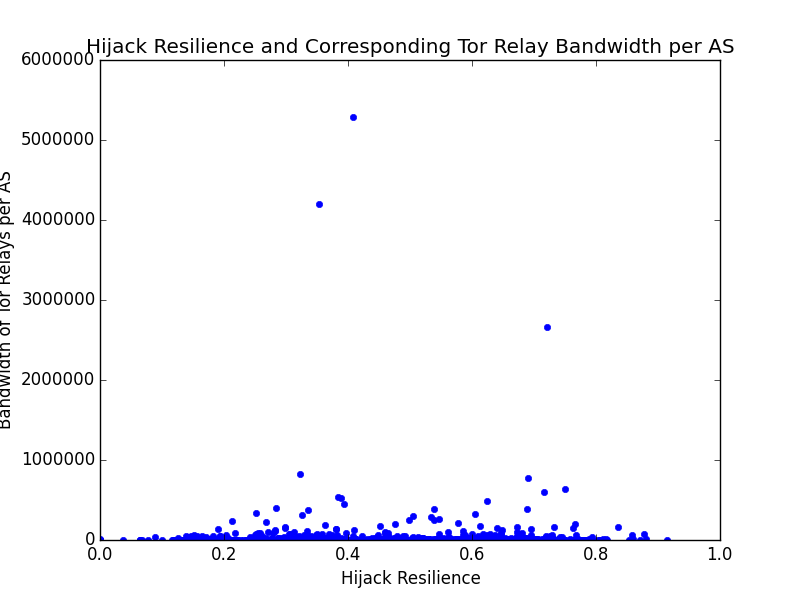
\includegraphics[width=\linewidth]{new_bandwidth}
  \caption{Hijack Resilience vs. Tor Bandwidth per AS}
  \label{fig:hijack_bw}
\end{subfigure}
\caption{Hijack resilience vs. relays/bandwidths for all Tor-related ASes.}
\label{fig:hijack_as}
\end{figure}

We can see that in both figures ~\ref{fig:res_relays} and ~\ref{fig:hijack_bw}, there is one significant outlier, AS16276 (OVH), which contains 339 relays and carries a total of 5,282,512 KB/s Tor bandwidths. It has a relatively low hijack resilience value of 0.408, indicating that in a hijack event, the probability of a Tor client (who uses relays in the AS) being deceived is close to 60\%. Another AS with high bandwidth yet low resilience is AS12876 (ONLINE S.A.S.), which contains 242 relays. It has an even lower resilience value of 0.35, and therefore, and even greater probability of being deceived by a hijack event. \\

%We then looked at which ASes had the most relays, and what their corresponding resilience is; ideally, ASes with more relays are also more resilient to hijack attacks.  Figure~\ref{fig:res_relays} shows the resilience value for an AS and the AS's corresponding number of relays.  

%\begin{figure}
%\centering
%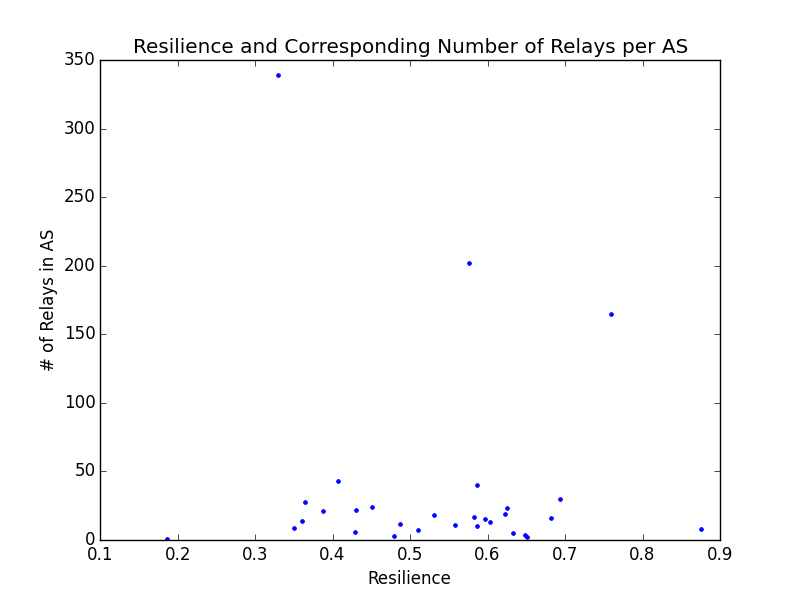
\includegraphics[width=.4\textwidth]{res_num_relays}
%\caption{Resilience values for each AS and each AS's corresponding number of relays.}
%\label{fig:res_relays}
%\end{figure}

%\begin{figure}
%\centering
%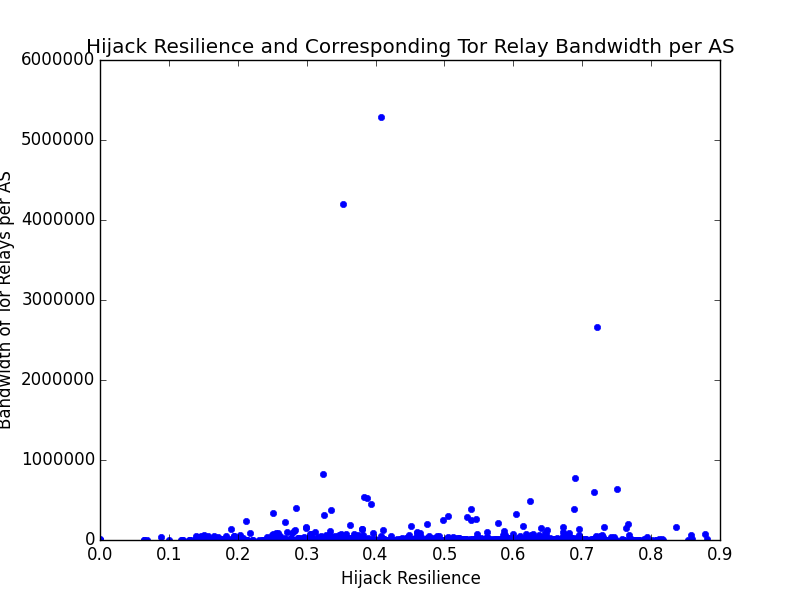
\includegraphics[width=.4\textwidth]{hijack_bandwidth}
%\caption{Bandwidth of all Tor relays in an AS, and the corresponding AS hijack resiliency.}
%\label{fig:hijack_bw}
%\end{figure}

%{\bf Resilience against Tier 1 ASes.} Tier 1 ASes play an important role in Internet routing and carry large amount of network traffic. Thus, we measured the resilience of Tor-related ASes specifically to Tier 1 ASes as hijacking ASes (instead of \emph{all} ASes). Figure~\ref{fig:resilience_histogram_tier1} shows the result. Surprisingly, 
%
%\begin{figure}[ht!]
%\centering
%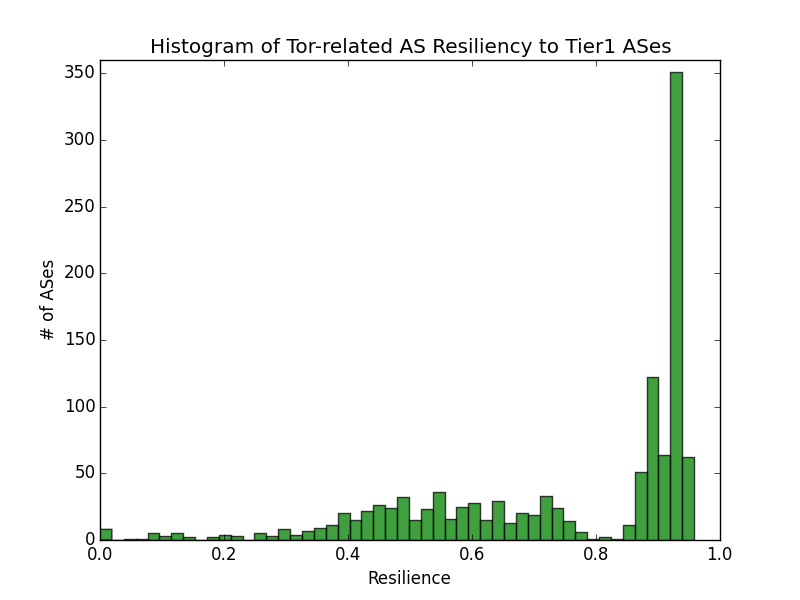
\includegraphics[width=.4\textwidth]{hijack_tier1}
%\caption{Histogram of hijack resiliences to Tier 1 ASes for all Tor-related ASes.}
%\label{fig:resilience_histogram_tier1}
%\end{figure}

{\bf Resilience over the years.} We also conducted our measurements on past data to analyze the hijack resilience trend on the Tor network.  Figure~\ref{fig:resilience_trend} shows the average AS resilience of Tor-related ASes to hijack attacks using January data from each year.  We can see that the average resilience has increased since 2008.  Note that the graph is drawn on a [0.43,0.49] scale, so the fluctuation in average resilience is relatively small. There was a slight decrease between 01/2013 and 01/2015, and then increased back again in 01/2016. After further investigation, we found that there was a steep increase in the number of Tor-related ASes from 2013 to 2015 - about 200 new ASes hosting Tor relays each year (18.8\% to 21.6\% increase), while the total number of ASes on the internet only increased marginally (0.26\% to 6.4\% increase). Thus, the corresponding decrease in average resilience might be due to many more stub ASes (potentially with low resilience values) starting to run Tor relays in those two years, which brought down the overall average. On the contrary, from 01/2015 to 01/2016, we saw an increase of $>6,600$ ASes in the internet (14.4\% increase), while the number of Tor-related ASes remained almost the same. A large portion of the new emerging ASes might be stub ASes with low hijacking influences, potentially resulting in the increase of total resilience values of the existing Tor-related ASes. 

\begin{figure}[ht!]
\centering
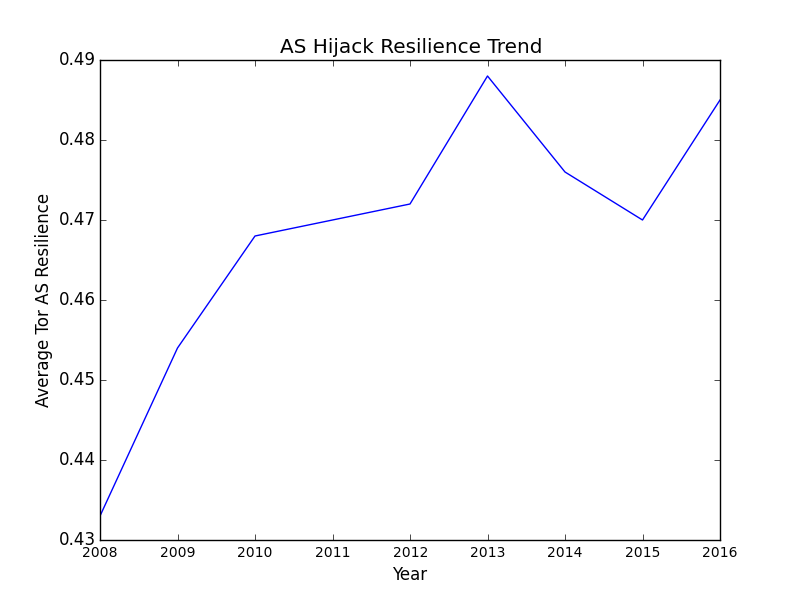
\includegraphics[width=.4\textwidth]{hijack_resilience_trend}
\caption{Average hijack resilience of Tor-related ASes each year from 2008 to 2016.}
\label{fig:resilience_trend}
\end{figure}

\subsection{Interception Resilience Results}

Tier-1 ASes play an important role in Internet routing. They sit at the top level of the internet hierarchy and carry a large amount of network traffic. Recall from the discussion in Section ~\ref{interception_methodology} that in order to successfully intercept traffic of a true origin AS, the false origin AS needs to satisfy a \emph{safe condition} - it cannot announce the invalid route to its providers when its existing route to true origin AS is through a provider route. This condition puts Tier-1 ASes at a powerful position - Tier-1 ASes do not have any providers and thus can always announce the invalid route to all its neighbors (peers/customers), which will be further propagated down to other ASes in the Internet hierarchy. On the contrary, ASes that are towards the bottom of the Internet hierarchy would not have much interception power. They have limited number of peers/customers, and most of their outgoing routes are through providers. Therefore, due to the difference in interception power, we only focus on measuring interception resilience to Tier-1 ASes as the attacking AS here instead of \emph{all} ASes as the attacking AS. 

We picked 17 ASes as Tier-1 ASes in our evaluation \footnote{AS174, AS209, AS286, AS701, AS1239, AS1299, AS2828, AS2914, AS3257, AS3320, AS3356, AS5511, AS6453, AS6461, AS6762, AS7018, AS12956}. We used the Tor consensus data and CAIDA Internet topology data, both from January 2016. Figure ~\ref{fig:interception_histogram} shows the distribution of interception resilience values of all Tor-related ASes. We can see that many Tor-related ASes have high resilience to interception attacks that could be carried out by Tier-1 ASes. The intuition behind this is that, even though Tier-1 ASes are at a position to intercept traffic, they also have longer paths from ASes that are close to the bottom of the hierarchy, which may prefer closer ASes with shorter paths instead of taking the longer paths to reach the Tier-1 ASes. 

\begin{figure}[ht!]
\centering
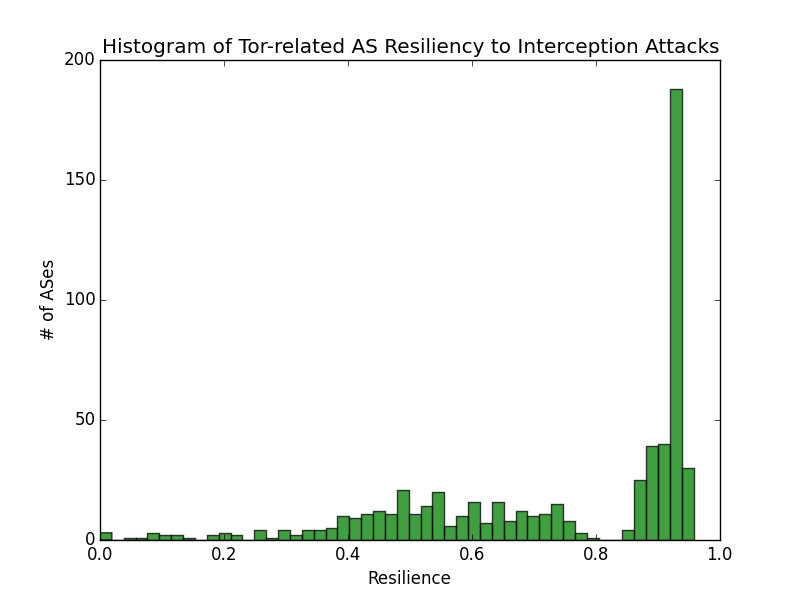
\includegraphics[width=.4\textwidth]{interception_resiliency}
\caption{Histogram of interception resilience values to Tier-1 ASes for all Tor-related ASes.}
\label{fig:interception_histogram}
\end{figure}

Figure ~\ref{fig:interception_bw} shows the plot of interception resilience values to Tier-1 ASes versus bandwidth of a Tor-related AS. Interestingly, the two ASes with highest Tor bandwidth - AS16276 (OVH) and AS12876 (ONLINE S.A.S.) - do not have high interception resilience. Their resilience values fall between 0.45 and 0.5, indicating that in an interception attack event by a Tier-1 AS, the probability of a Tor client (who uses relays in either of these two ASes) being deceived is $> 50\%$. Note that this result is consistent with the hijack resilience result shown in Figure ~\ref{fig:hijack_bw}, with these same two ASes of high bandwidth yet low resilience values. 

\begin{figure}[ht!]
\centering
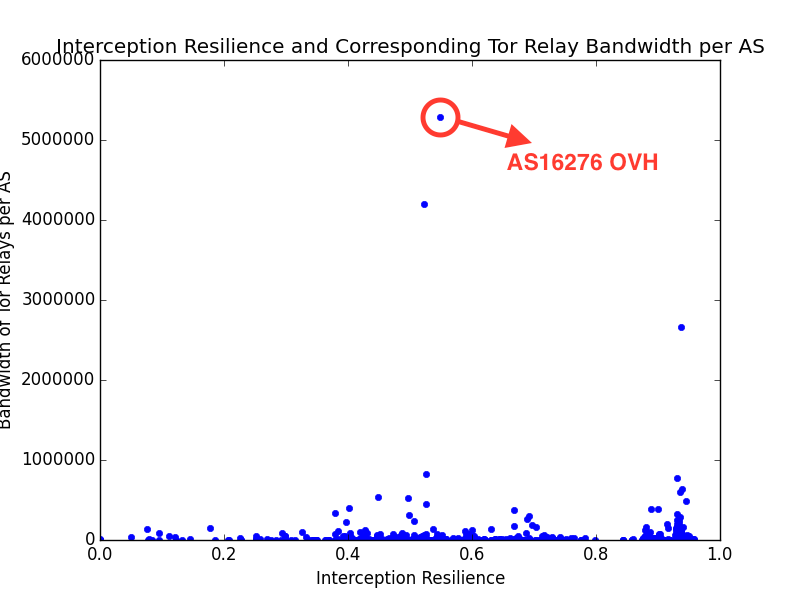
\includegraphics[width=.4\textwidth]{interception_bandwidth}
\caption{Interception Resilience to Tier-1 ASes vs. Tor Bandwidth per AS}
\label{fig:interception_bw}
\end{figure}

%\subsection{Case Study: Indosat 2014}
%In 2014, Indosat, one of Indonesia's largest telecommunications networks, announced 417,038 new prefixes, but it usually only announces about 300 prefixes~\cite{indosat2014}.  Previous work found that this compromised 44 Tor relays, 38 of which were guard relays and 17 of which were exit relays (11 hijacked relays were both guards and exits) ~\cite{sun2015raptor}.  We calculated the hijack resilience of the hijacked ASes; the results are shown in Figure~\ref{fig:case_study}.  We can see that the AS hijack resilience values range from 0.0 to .76, with most ASes falling in the middle of the spectrum. 
%This means that even ASes with relatively high resilience values (.72 and .76) have the potential to be hijacked.  

%\yixin{Should we omit this subsection completely? The intention was to validate our metric by doing a case study, but it does not seem to serve the purpose without going into more details. Plus, a better way to validate the metric might be to perform a hijack attack ourselves using transit portal and evaluate the affected ASes vs. their resilience values. However, we do not have the TP ready and thus cannot perform this experiment now.}

%\begin{figure}
%\centering
%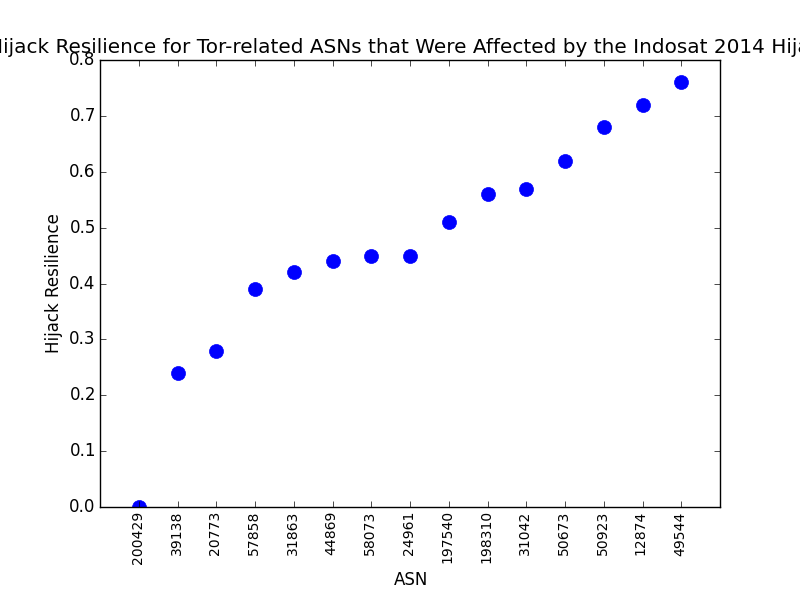
\includegraphics[width=.4\textwidth]{case_study_graph}
%\caption{The ASes that contain at least one Tor relay, and were affected by the Indosat hijack attack in 2014, along with their corresponding hijack resiliency values.}
%\label{fig:case_study}
%\end{figure}

{\bf Bandwidth is not enough.} We have shown in this section that Tor-related ASes with high bandwidth can have low resilience values to both hijack and interception attacks, and thus are more likely to be susceptible to active BGP attacks compared to high resilience ASes. What's even worse is that high bandwidth relays are more preferred by Tor users during relay selection, resulting in exposing many Tor users to the high risk of being compromised by active BGP attacks. Therefore, this vulnerability motivates our work on incorporating AS resilience into relay selection, which we will delve into details in Section ~\ref{subsec:relayselection}.



